\documentclass[a4paper,DIV=12,english]{scrartcl}
\usepackage[utf8]{inputenc}
\usepackage{graphicx}
\usepackage{hyperref}
\usepackage{csquotes}
\usepackage{amsthm}
\usepackage{amssymb}
\usepackage{bbm}
\usepackage{amsmath}
\usepackage{tikz}
\usepackage{svg}
\usepackage{braket}
\usepackage{caption}
\usepackage{subcaption}
\usepackage{placeins}
\usepackage[backend=bibtex]{biblatex}
% Fakesection
\newcommand{\fakesection}[1]{%
    \par\refstepcounter{section}                                        % Increase section counter
    \sectionmark{#1}                                                    % Add section mark (header)
    \addcontentsline{toc}{section}{\protect\numberline{\thesection}#1}  % Add section to ToC
    % Add more content here, if needed.
} 

\renewcommand{\thesubsection}{\thesection.\alph{subsection}}

\title{Data and Signal Analysis\\Problem Sheet 4}
\author{Elise Pilgermann, Max Maschke}
\date{\today}

\begin{document}
\maketitle

\section{Windowing}

\section{Empirical Mode Decomposition}
\begin{figure}
    \centering
    \begin{subfigure}{0.49\textwidth}
        \centering
        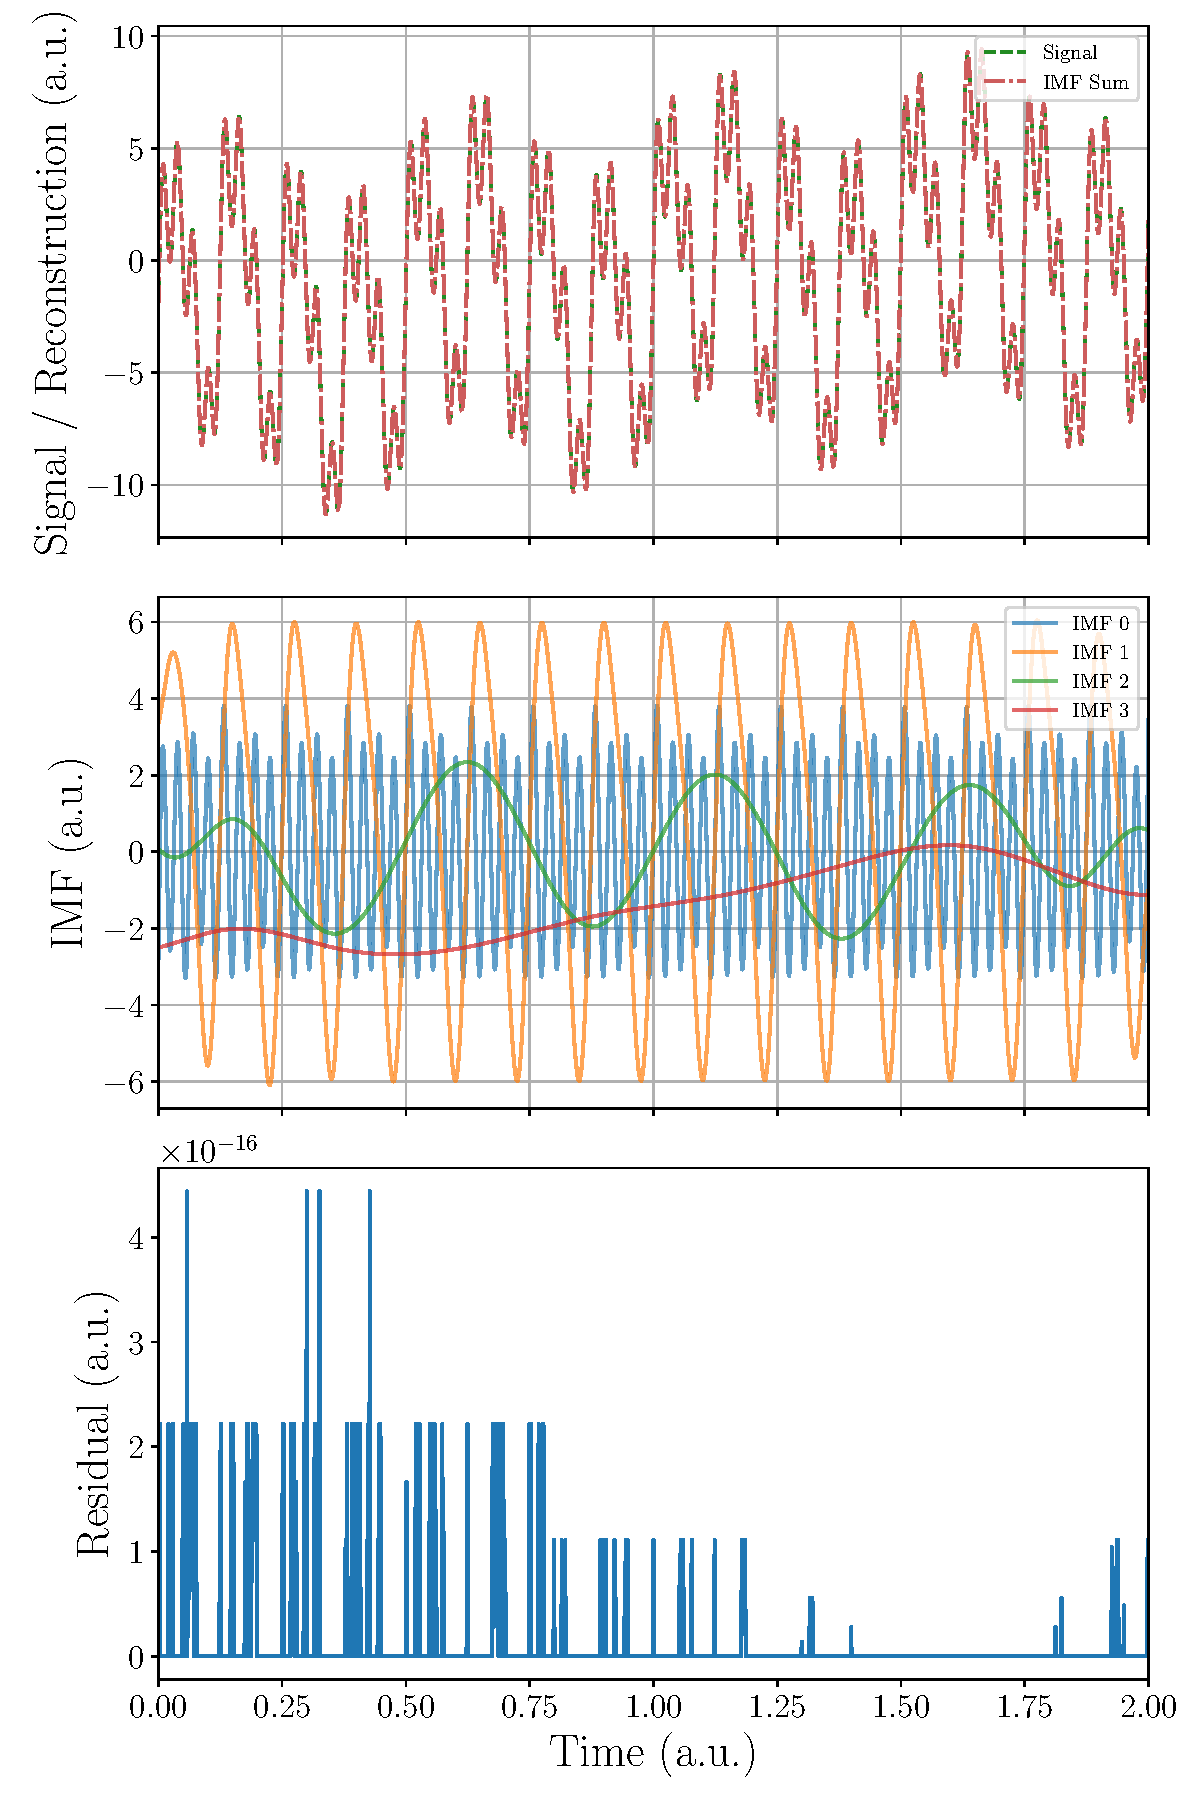
\includegraphics[width=\textwidth]{../imf.pdf}
        \caption{}
        \label{subfig:imf}
    \end{subfigure}
    \begin{subfigure}{0.49\textwidth}
        \centering
        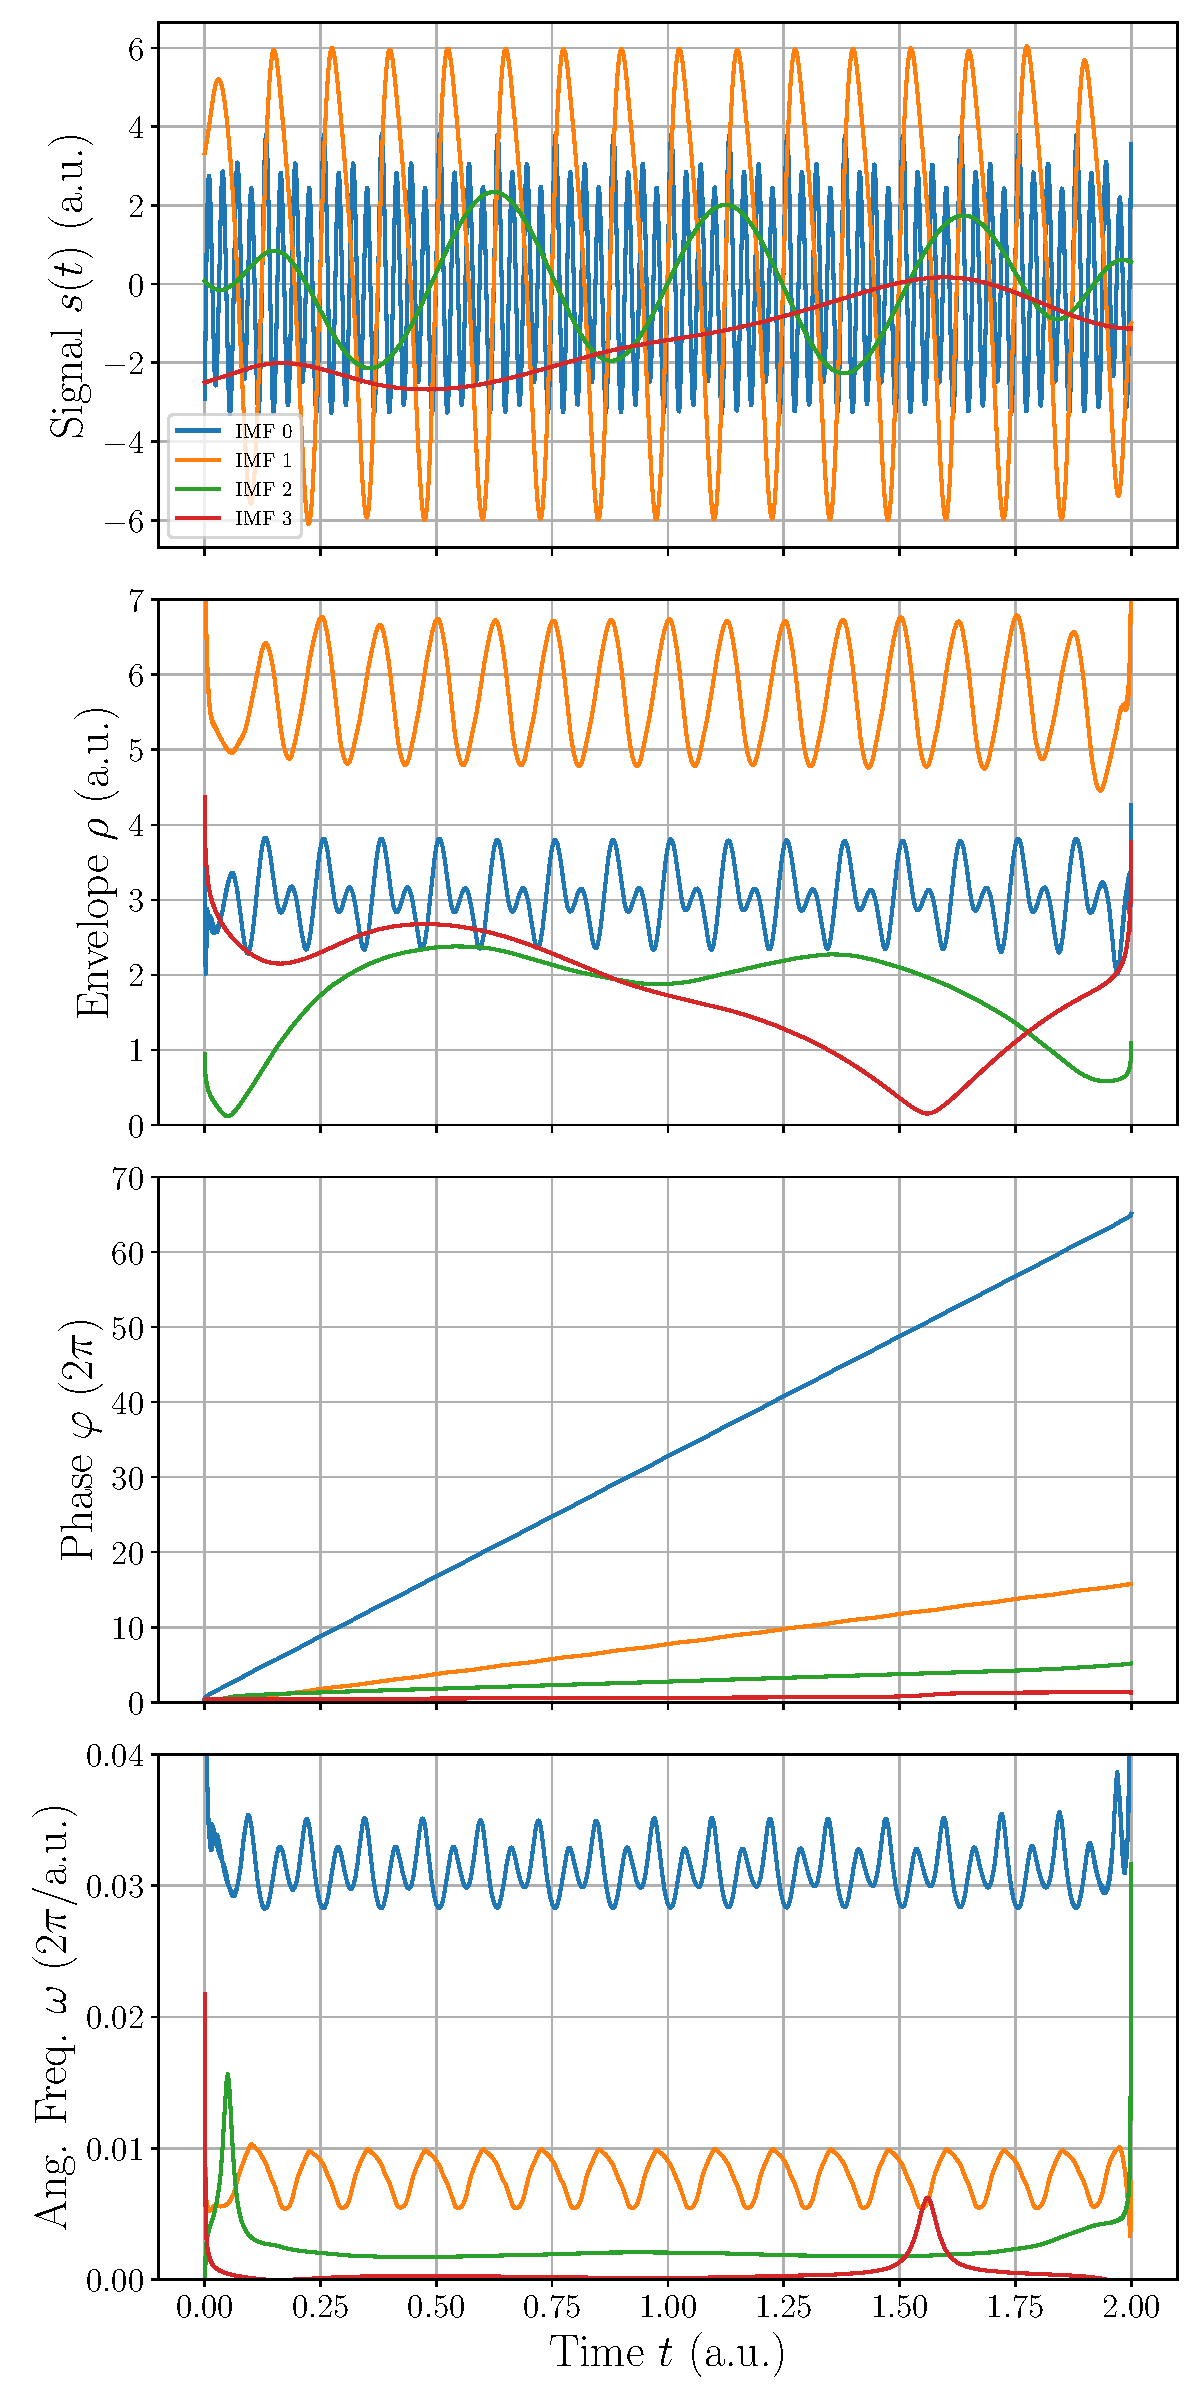
\includegraphics[width=\textwidth]{../imf_analytic_sig.pdf}
        \caption{}
        \label{subfig:as}
    \end{subfigure}
    \caption{}
    \label{fig:imf}
\end{figure}

\section{Method of Least Squares}

\begin{figure}
    \centering
    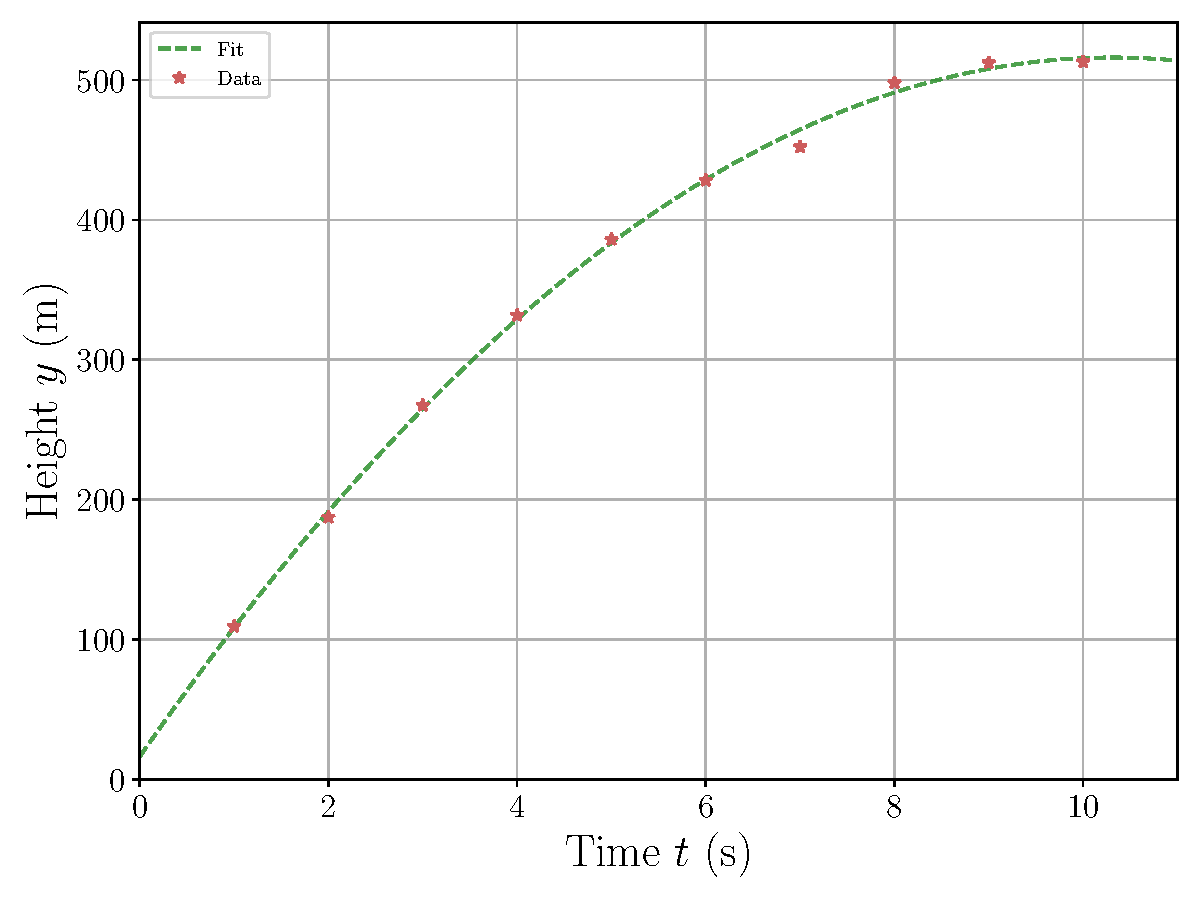
\includegraphics[width=0.7\textwidth]{../lstsq.pdf}
    \caption{}
    \label{fig:lstsq}
\end{figure}

\end{document}